%!TEX root = ../dissertation.tex

\chapter{BlendMe!}
\label{chapter:design}

\section{Objectives}
\label{sec:impl_objectives}
%
As seen before, there is a myriad of questions about the usage of color blendings when conveying information, which remained unanswered. However, only a set of questions
is answered in our research, since it is not possible to reach answers to all questions. Therefore, the goals which we have picked for this User Study are as follows:
%
\begin{enumerate}
	\item Study a way to present color which does not influence color perception.
  \item Understand if there is any psychological organization of color, when detailing color mixtures' components.
  \item If possible, obtain results to ascertain the cultural influence in color perception.
  \item Study the influence of discrete and continuous color scales.
\end{enumerate}
%
Additionally, it is relevant to understand which color model stands as the best to mix colors which are, from a perceptual point of view, more similar to the users expectation.
We have planned to develop this study in two different strands: in a \textbf{Laboratory Environment}, which will allow us to calibrate and perfectly control the entire study conditions,
and in an \textbf{Online Environment}, which will allow us to disseminate our study to a larger set of users, even without controlling the calibration of the testing environment). \par
%
The questions which we think define our research goals, for this study, are:
%
\begin{itemize}
	\item \textbf{Q1:} Which Color Model meets best the users' expectations, when blending two colors?
	\item \textbf{Q2:} Is there evidence of a spatial arrangement of colors, when users are indicating possible color mixtures' results?
	\item \textbf{Q3:} Are there evidences from differences across demographic groups, such as the age or gender?
\end{itemize}
%
Along the result analysis, each question will meet its answers. These questions will be explored in multiple threads, such as:
%
\begin{enumerate*}
		\item \textbf{Analyzing the distances of each answer pair to the ideal answers of each color model}, verifying which color models had the best and the worst
		values yielded by the descriptive statistic analysis,
		\item \textbf{Evaluate the results from blendings when the basis is given to the user, against when the result of the blending is given},
		\item \textbf{Verify if the color models which have the best and worst results are subtractive or addictive},
		\item \textbf{Analyze the ease of blending colors}, or if
		\item \textbf{There is substantially different results among genders, or different age groups}.
\end{enumerate*}
\\ \\
%
Justificar nome \\
Referir HSL com hue variante, e SL com parametros maximos. \\

To meet these study requirements, we drafted our study into three different phases: a \textbf{User Profiling Phase}, a \textbf{Calibration Phase}, a \textbf{Color Deficiency Test Phase} and finally, the \textbf{Core Phase}. In the following sections, we detail each of these sections. \par
%
\section{Designing the Solution}
\label{sec:impl_designingsolution}
Design the implementation, talk about the process ever since wireframing, through the mapping of concepts between
what we want and how we implemented, in order to achieve what we want. Include screenshots from the implementation. \\

Important detail: color conversion between Excel and adapted colors with ICC profile, Spyder and all. ColorConverter.m. \\
%
Dividir secção em partes do estudo, introduzindo com Research Proposal para motivar decisões. Referir todos os detalhes de implementação.
Justificar completamente todas as decisões que foram tomadas (número de placas, informações pedidas, métricas colhidas, tudo.)
%
Falar de folha de calculo do excel com todas as cores, que depois for migrada para matlab
e convertida de acordo com perfil de calibração.

One of the points discussed in section \ref{sec:background_discussion} was the amount of users who performed the study of Gama and Gonçalves
\cite{Gama20141,Gama20142}: it was large enough for their questions. However, considering the results we aim to achieve with this study, a considerably larger sample of users is the ideal: besides conducting
the study in a laboratory environment, it is mandatory to expand the sample size by performing user studies with online users, trying to take advantage of
the cultural diversity that may arise. These online answers will become from online users from social networks, in which we will spread our study in a \emph{word-of-mouth} scheme. \par




%
\subsection{User Profiling Phase}
\label{subsec:design_profiling}
%
\textbf{FALTA TEXTO AQUI...} \par
%
In this phase of the study, questions about the Age, Gender, Academic Degree, Nationality, Country of Residence and the Native Language of the user should be asked: these questions will help us conceiving user profiles with key indicators about cultural background and gender relation to results of each test. \par
%
\textbf{\underline{\emph{(... ACRESCENTAR AQUI MAIS INFOS RELEVANTES ...)}}} \par
%
When this phase is concluded, the user will be guided to another stage of the study, to perform the \textbf{Calibration Phase}, where he will be asked to analyze a set of images and answer a pair of questions. \par
%
\subsection{Testing Calibration Phase}
\label{subsec:design_calibration}
%
Performing online tests - specially when trying to obtain precise values about color - carries obvious problems on how it is guaranteed the results which may appear are, in fact, compliant with certain patterns of
quality, specially color and monitor calibration patterns. \par
%
To overcome this problem, the ideal solution is to develop a system capable of acquiring information about the user's monitor calibration, \emph{e.g.} Brightness, Contrast, RGB Color Balance, Gamma or Saturation, as a pre-step of the study and apply an appropriate calibration when rendering the study's main page. Since we have not found a way to tackle this solution so far, we developed another solution: to present, as pre-step, some calibration images in which the user will have to perform a set of small tasks, indicating us a set of answers; in the end of the test, we have to analyze the answers to verify if they are compliant with a certain pattern of calibration acceptability, determining if the answers of a certain user can be considered true and not misleading. \par
%
\begin{figure}[!ht]
	\centering
  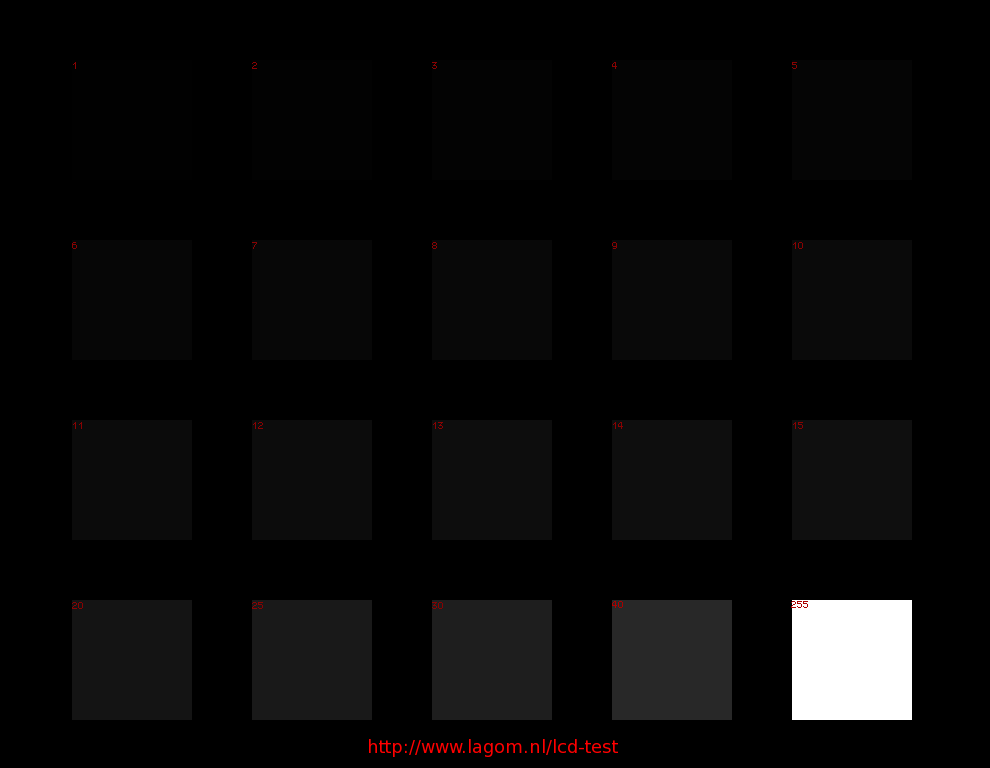
\includegraphics[width=0.35\textwidth]{images/blacktest_example.png}
  \caption[Black Squares Test]{Example of Black Squares Test.\protect\footnotemark{}}
  \label{fig:blacktest_example}
\end{figure}
\footnotetext{"Black Level", Available at: \url{www.lagom.nl/lcd-test/black.php}. Last accessed on September 7th, 2016.}
%
We will present to the user a \textbf{pair of images}, consisting of a set of 10 squares each; in the first of them, we will test the black level of user's monitor, showing each square with a different shade of black, from brighter ones (Square 1) to darker ones (Square 10). The user is, then, asked to express which square is the last, most perceivable, darker square, and point out the word which follows it. The second image has the same job as the first one, except that this rules out the white-level of the monitor and the ten squares present different tones of white. An example of this sort of test is presented in Figure \ref{fig:blacktest_example}. The results of this phase are recorded for further analysis when the study finishes. \par
%
Regarding the laboratory environment, we are going to conduct the user tests in a LCD monitor, under a fixed light source; the monitor will be calibrated
using a colorimeter which will consider the existing light in the environment and adjust the color of each pixel to a standard. The user will be focused on
the task and no other user will be present in the room at the same time, excluding the study regulator; the user will have a fully detailed test protocol to
follow.
%
\textbf{\underline{\emph{(... FALTA TEXTO AQUI ...)}}}
%
Referir limitação descoberta entre Chrome Safari
%
\subsection{Testing Color Vision Deficiencies Phase}
\label{subsec:design_ishihara}
%
\subsection{Core Test Phase}
\label{subsec:design_core}
%
Incluir tabela com todas as cores, igual a folha de auxilio. Referir que Ciano, por erro, não esta a ser testado no formato objTwoColors. \\
Referir aqui que dados estão a ser guardados do utilizador, e como estão a ser guardados, (objTwoColors e twoColorsObj), etc.
Referir aqui também que slider contemplava cores standard da folha de calculo para ambiente online,
mas para ambiente laboratorio cores eram antes processadas no Matlab. Slider não tinha cores ordenadas para que utilizador não utilizasse
algum modelo mental e aprendesse previamente a misturar. Cores foram misturadas sem qualque critério (referir ordem pela qual apareciam).
Referir aqui caminho do calibrador -> icc -> matlab -> converter cores -> slider


%
\begin{table}[htbp]
  \resizebox{\textwidth}{!} {
  \begin{tabular} {|c|c|c|c|c|c|c|c|c|c|}
    \hline
    User ID & Type & First Color & Second Color & Third Color & Drags & Time & Rating & Resets & Question ID \\ \hline \hline
    5710cca334d60 & objTwoColors & \#0080FF & hsl(58.69565217391305,1,0.50) & hsl(98.15217391304348,1,0.50) & 992 & 117 & 4 & 2 & 10 \\ \hline
    5745c1c07cc0c & objTwoColors & \#8000FF & hsl(300,1,0.50) & hsl(324.13043478260875,1,0.50) & 645 & 55 & 2 & 1 & 14 \\ \hline
    5745350dc1e22 & objTwoColors & \#0080FF & hsl(226.30434782608697,1,0.50) & NONE & 115 & 11 & 5 & 1 & 10 \\ \hline
    57451c3b38192 & objTwoColors & \#00FF80 & NONE & hsl(150,1,0.50) & 462 & 39 & 5 & 1 & 15 \\ \hline
    574511e99b6d9 & objTwoColors & \#0080FF & hsl(15.652173913043478,1,0.50) & hsl(316.30434782608694,1,0.50) & 442 & 40, & 1 & 1 & 10 \\ \hline
    57427cf6bad0c & twoColorsObj & \#00FFFF & \#FFFF00 & \#46FF9C & 6 & 14 & 3 & 1 & 32 \\ \hline
    5740bda9be3dc & objTwoColors & \#FF7200 & hsl(9.130434782608695,1,0.50) & hsl(50.21739130434783,1,0.50) & 45 & 22 & 5 & 1 & 11 \\ \hline
    573c783748e8b & twoColorsObj & \#00FFFF & \#CBFF00 & \#00FF6B & 44 & 25 & 3 & 1 & 32 \\
    \hline
  \end{tabular}}
  \caption[Excerpt of Raw "Results" Table]{Excerpt of Results Table, with raw data.}
  \label{table:csv_resultsraw}
\end{table} \par
%

%
\section{Evaluation Criteria}
\label{sec:impl_evaluationcriteria}
Ishihara plates and more, whatever we consider relevant. Falar também de como a calibração era considerada válida ou não. Erros
que poderiam ser gerados pelo field number html5, que com scrolls podia dar valores errados. \\
